% ===================================================================
\chapter{Evaluation Method}
\label{ch:evaluation}

This chapter sets out how the methods of Chapter~\ref{ch:methods} were
evaluated: the two stages of the evaluation, the signal chain that produces
their input, the metrics, and the verification ladder that carries every
result from MATLAB down to the FPGA board.

\section{Two stages}
\label{sec:stages}

The evaluation runs in two stages, each answering one question.

\paragraph{Stage 1 --- which methods are worth building?}
All eight methods of Section~\ref{sec:candidates} are run in MATLAB over the
same 50 consecutive ColoRadar frames with all 16 receive channels. Each is
scored on compression ratio and on what it does to target detection. A method
goes forward only if it is lossless --- it loses no detections beyond those of
the FX16 step every method shares --- and compresses by more than three, which
leaves a margin over the \num{2.4}--\num{2.7} that a Gigabit Ethernet link needs
(Section~\ref{sec:kiem}).

\paragraph{Stage 2 --- where does the compression come from, and what does it
cost in hardware?}
The selected methods, DRHE and LPC, are evaluated on the four-receiver frames
that the hardware processes. Their compression ratio is broken down into what
the entropy coder achieves alone, what prediction adds, and what a re-derived
dictionary adds. They are then implemented, with decoders, in hardware
(Chapter~\ref{ch:hardware}), verified bit for bit at every level of the ladder
of Section~\ref{sec:ladder}, and measured on the board for time per frame,
latency and chip resources.

\section{The reference signal chain}
\label{sec:refchain}

The MATLAB chain is described here in the order it executes, because several
later observations depend on details of individual steps.

\subsection{Loading}
A frame is read from the ColoRadar binary and reshaped into a complex cube of
(fast time $\times$ ramp $\times$ receiver), with the TDM flattening of
Equation~\eqref{eq:rampindex}. The per-ramp mean is subtracted from each
channel to remove the DC / transmitter-leakage term.

\subsection{Windowing}
A Hann window is applied along fast time to suppress spectral leakage, so that
a strong nearby target does not bury a weak distant one in sidelobes.

\subsection{Range FFT}
An $N_s$-point FFT is taken along fast time and normalised by $N_s$. Only the
positive half-spectrum is retained, giving $N = 128$ range bins. This halving
is a deliberate choice, not a consequence of conjugate symmetry --- the input
here is complex $I/Q$, so the spectrum is \emph{not} symmetric; the negative
half corresponds to negative beat frequencies, which are not physically
meaningful ranges.

\subsection{FX16 quantisation}
The complex FFT output is scaled by Equation~\eqref{eq:scale} and rounded to
\texttt{int16}. This is the last step before compression, and its output ---
128 range bins $\times$ 192 ramps $\times$ 4 receive channels of complex
\texttt{int16} --- is exactly what both compressors consume.

Four receive channels rather than sixteen are exported to the hardware path,
because four complex \texttt{int16} samples is \num{128} bits, the AXI4-Stream
width. One such frame is $128 \times 192 \times 4$ complex samples, or
\SI{393216}{\byte}; the 50-frame test set is \SI{19.7}{\mega\byte}.
Figure~\ref{fig:input} shows one receiver of one such frame.

\begin{figure}[htbp]
\centering
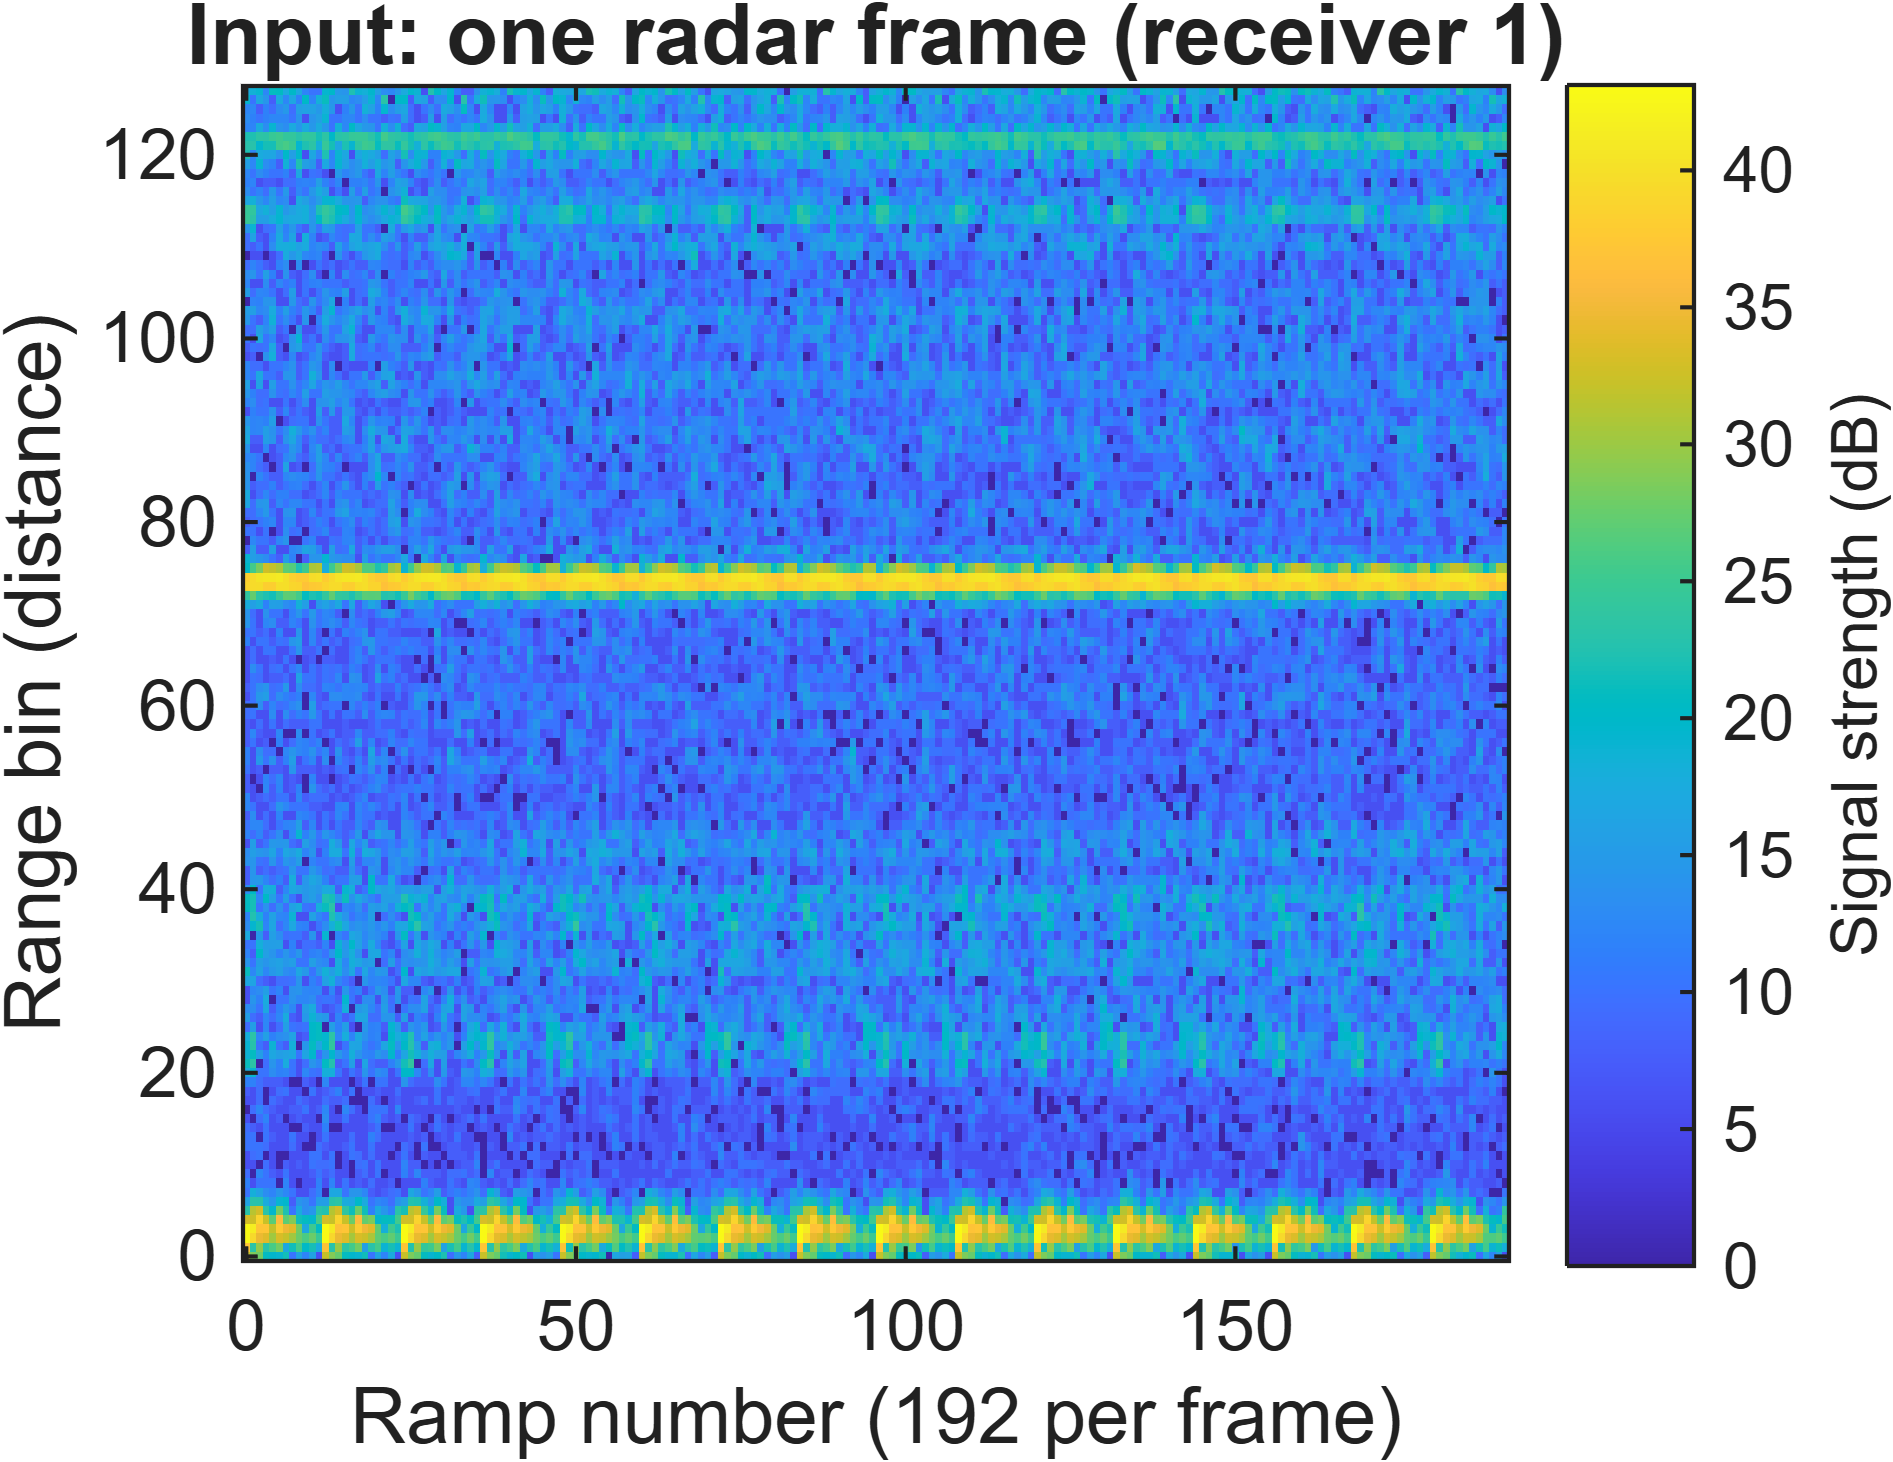
\includegraphics[width=0.6\textwidth]{fig_input.png}
\caption[One input frame]{One input frame as the compressor receives it:
receiver 1 of ColoRadar frame 0 after the range FFT and FX16 quantisation, 128
range bins by 192 ramps. Strong returns appear as horizontal bands at fixed
range; most of the frame is low-level noise, which is why it compresses.}
\label{fig:input}
\end{figure}

\subsection{Detection and metrics}
The reconstructed data is put through a Doppler FFT and a threshold detector,
and the resulting detections are compared against those from the
double-precision reference. Three details of this chain matter for how its
results should be read:

\begin{itemize}
\item the Doppler FFT is a 192-point FFT across \emph{all} ramps of the frame,
in the order they were recorded --- that is, across the transmitter-interleaved
ramp axis of Section~\ref{sec:tdm}, not across the 16 ramps of any one
transmitter;
\item there is no angle FFT: the 16 receive channels are combined by
non-coherent integration (summing magnitudes), so ``detection'' here means a
peak in a range--Doppler map, not a localised point in space;
\item the threshold is the mean of the lowest \SI{75}{\percent} of sorted
magnitudes plus a fixed \SI{15}{\decibel} offset, with 8-connected
local-maximum suppression.
\end{itemize}

\noindent
Neither of the first two affects any lossless result, since a lossless
compressor returns the input exactly and every downstream stage then agrees by
construction. They matter only for the lossy comparison points, whose detection
losses are measured by a chain that is simpler than a production one
(Section~\ref{sec:threats}).

\section{Metrics, defined precisely}
\label{sec:metrics}

Several metric names are used loosely in this field. They are pinned down here.

\subsection{Compression ratio}
\begin{equation}
\mathrm{CR} = \frac{B_{\mathrm{in}}}{B_{\mathrm{out}}},
\qquad
B_{\mathrm{in}} = N_{\mathrm{ramps}} \times N \times N_{\mathrm{RX}} \times 32,
\end{equation}
with $B_{\mathrm{out}}$ the compressed length \emph{including} AXI packet
padding. Including the padding matters: a design that flushed its bit buffer
per ramp rather than per frame would waste up to 255 bits per ramp, costing
about \SI{2.9}{\percent} of the ratio. Reporting the ratio without padding
would hide that design choice. Ratios are computed per frame and reported as
the mean over the 50 frames; the ratio of the totals differs by about
\SI{0.2}{\percent} (for example \num{4.208} against a mean of \num{4.217} for
DRHE).

\subsection{Maximum absolute difference}
\begin{equation}
\mathrm{MaxDiff} = \max_{\text{all samples}}
   \bigl| x - \tilde{x} \bigr|
\end{equation}
over every real and imaginary component. For a lossless coder the pass
criterion is $\mathrm{MaxDiff} = 0$. There is no tolerance.

\subsection{Detection metrics}
\label{sec:detectionmetrics}

Let $D_{\mathrm{ref}}$ be the detection set from the double-precision reference
and $D_{\mathrm{test}}$ that from the reconstructed data. The two rates reported
are
\begin{equation}
\mathrm{FN}\% = \frac{|D_{\mathrm{ref}} \setminus D_{\mathrm{test}}|}{|D_{\mathrm{ref}}|},
\qquad
\mathrm{FP}\% = \frac{|D_{\mathrm{test}} \setminus D_{\mathrm{ref}}|}{|D_{\mathrm{test}}|}.
\end{equation}

The first is a false negative rate in the ordinary sense: the share of real
targets that are missed, reported as \emph{missed targets}. The second is
labelled a false positive rate in Kiem's thesis, but it normalises by the
number of \emph{test detections} rather than by the number of true negatives,
which makes it a \textbf{false discovery rate} (FDR): the share of reported
detections that are spurious. It is reported under that name here.

Two further properties bound how much weight the detection metrics can carry,
and are stated rather than buried:

\begin{itemize}
\item \textbf{The comparison is cell-wise and exact.} A target detected one
range--Doppler cell away from its reference position counts as both a false
negative \emph{and} a false discovery. There is no positional tolerance, which
inflates both rates relative to a matched-detection criterion.
\item \textbf{The \SI{15}{\decibel} threshold is a free parameter.} It is not
swept, and the detection rates are sensitive to it.
\end{itemize}

\subsection{What the detection metrics actually measure here}

This point is important enough to state on its own. FX16, DRHE and LPC are all
exactly lossless \emph{with respect to the FX16 codes}. Their reconstructed
data is bit-identical, so their detection metrics are identical \emph{by
construction} --- not by coincidence, and not as evidence that the compressors
are equally good.

What the detection metrics measure for the lossless methods is therefore the
cost of the \textbf{FX16 quantisation step}, which is the only lossy operation
in the lossless chain. For the lossy methods they measure the cost of
quantisation and compression together.

\subsection{No-prediction baseline and order-0 entropy}
To separate what the predictor contributes from what the entropy coder
contributes, every predictive result is reported against a \emph{no-prediction
baseline}: the FX16 codes fed straight into the same entropy coder. A predictor
that does not beat it is not helping, however good the overall ratio looks. In
the same spirit, Equation~\eqref{eq:entropy} is evaluated empirically on the
residual distribution: the entropy is the figure of merit for the
\emph{predictor}, and the gap between it and the achieved bits per value is the
inefficiency of the \emph{dictionary}.

\subsection{Timing}
Three timing quantities are reported for the hardware, and they answer
different questions.
\begin{itemize}
\item \textbf{Time per frame}: clock cycles from the start of a frame's DMA
transfer to the last output word being written, divided by the clock. It sets the frame rate the
design can sustain.
\item \textbf{Throughput}: input bits per frame divided by the time per frame.
\item \textbf{End-to-end latency}: the time from the last input word being read
from memory to the last output word being written back, measured by the board
firmware with a hardware timer. This is Kiem's definition, and it measures how
long the compressed data lags the raw data --- the quantity that matters for a
sensor feeding a real-time system.
\end{itemize}
For a streaming design latency is a small fraction of the time per frame; for
a design that must see the whole frame first, it is most of it.


\section{The verification ladder}
\label{sec:ladder}

A compressor that is \emph{nearly} lossless is useless, so the method has to
prove exactness rather than estimate it. Every design is therefore taken down
a ladder of five levels, each checked against the one above it, so that a
discrepancy always localises to a single transition (Figure~\ref{fig:ladder}).

\begin{figure}[t]
\centering
\begin{tikzpicture}[font=\small,
  ph/.style={draw=accent,line width=1pt,fill=lightbg,rounded corners=2pt,minimum width=40mm,minimum height=11mm,align=center,font=\scriptsize},
  a/.style={-{Latex[length=1.6mm]},slate}]
\node[ph] (p1) at (0,0)    {\textbf{1. MATLAB}\\double-precision reference};
\node[ph] (p2) at (0,-1.6) {\textbf{2. HLS C-simulation}\\the C++ run as software};
\node[ph] (p3) at (0,-3.2) {\textbf{3. RTL co-simulation}\\the synthesised hardware};
\node[ph] (p4) at (0,-4.8) {\textbf{4. Vivado implementation}\\placed and routed};
\node[ph] (p5) at (0,-6.4) {\textbf{5. KCU116 board}\\the real system};
\draw[a] (p1) -- (p2); \draw[a] (p2) -- (p3); \draw[a] (p3) -- (p4); \draw[a] (p4) -- (p5);
\node[font=\scriptsize,text=slate,anchor=west,align=left] at (2.5,0)
  {all eight methods; exact bit counts,\\detection metrics};
\node[font=\scriptsize,text=slate,anchor=west,align=left] at (2.5,-1.6)
  {does the C++ reproduce MATLAB \emph{bit for bit}?\\does the decoder recover every sample?};
\node[font=\scriptsize,text=slate,anchor=west,align=left] at (2.5,-3.2)
  {does synthesis preserve it?\\cycle-accurate latency};
\node[font=\scriptsize,text=slate,anchor=west,align=left] at (2.5,-4.8)
  {routed resources and timing\\for the whole system};
\node[font=\scriptsize,text=slate,anchor=west,align=left] at (2.5,-6.4)
  {output byte-identical to C-simulation?\\measured time, throughput, latency};
\end{tikzpicture}
\caption[The verification ladder]{The verification ladder. Each level is checked
against the one above it, so a mismatch localises to a single transition rather
than to ``somewhere in the design''.}
\label{fig:ladder}
\end{figure}

\paragraph{Level 1 --- MATLAB.}
The whole radar chain is modelled in double precision and every method is run
against it. This establishes the golden reference: the exact FX16 values, the
exact number of bits each algorithm should produce, and the detection metrics.

\paragraph{Level 2 --- HLS C-simulation.}
Because the hardware is written in C++, it can be compiled and run as ordinary
software. This level asks whether the C++ produces \emph{exactly} the bits
MATLAB says it should, and whether the decompressor recovers \emph{exactly} the
original samples, over all 50 frames. It runs in minutes. The stimulus is
exported from MATLAB as \texttt{int16} rather than recomputed in C++, so both
environments operate on byte-identical input and any difference in output is
unambiguously a difference in the compressor.

\paragraph{Level 3 --- RTL co-simulation.}
The C++ is synthesised to Verilog and the same testbench is re-run against the
generated RTL. This checks that synthesis preserved behaviour --- pipelining,
array partitioning and fixed-point inference can all change results if a
design is subtly wrong --- and gives a cycle-accurate latency figure.
Co-simulation is run on one frame, since the per-frame behaviour is
deterministic and 50 frames of RTL simulation with floating-point IP take many
hours.

\paragraph{Level 4 --- Vivado implementation.}
Each core is packaged as IP and built into the complete board system
(Section~\ref{sec:system}), then synthesised, placed and routed by Vivado. This
replaces the HLS resource and clock \emph{estimates} with the figures of a real
netlist: post-route utilisation per core and for the whole system, and the
worst timing slack at \SI{100}{\mega\hertz}.

\paragraph{Level 5 --- the board.}
The bitstream runs on an AMD KCU116 evaluation board. All 50 frames are
streamed through the compressor by DMA, the compressed output is compared byte
for byte with the C-simulation output, the decompressed output is compared with
the original frames, and the firmware times every frame with a hardware timer.

\section{Edge-case testing}
\label{sec:edgecases}

Real data exercises the typical case well and the extreme case not at all. The
ColoRadar residuals span roughly $[-514, +416]$, which is entirely inside
category 10 of a 16-category code. Everything above that is never exercised by real data.

An eight-case synthetic testbench was therefore built
(Table~\ref{tab:edgecases}), generating its stimulus internally so that it runs
identically in C-simulation and co-simulation.

\begin{table}[t]
\centering
\caption[Synthetic edge cases]{The synthetic edge-case suite. Each case has its
own allowed reconstruction error --- zero for all but the three that can
produce the value $-32768$ and therefore exercise the saturation described in
Section~\ref{sec:robust}. Uniformly random \texttt{int16} input produces a
residual of $-32768$ by chance, so it is one of them.}
\label{tab:edgecases}
\small
\begin{tabular}{@{}llc@{}}
\toprule
Case & What it exercises & Allowed $\mathrm{MaxDiff}$ \\
\midrule
all-zeros        & the $S_4 = 0$ path and the best case & 0 \\
dc-constant      & a perfectly predictable sequence & 0 \\
random-int16     & the worst case: incompressible input & 1 \\
tone-192ramp     & a periodic sequence the AR model should fit & 0 \\
tone-1ramp       & a sequence too short to fit & 0 \\
max-amplitude    & full-scale values, and 128-bit correlations & 0 \\
max-alternating  & $\pm 32767$ alternating: the largest residuals & 1 \\
int16-min        & $-32768$ specifically & 1 \\
\bottomrule
\end{tabular}
\end{table}

The suite exercises the parts of the design that real data never reaches,
including the two situations handled by the robustness measures of
Section~\ref{sec:robust}, neither of which can arise on ColoRadar data.

\section{An independent implementation}
\label{sec:indep}

As a final check that the compression figures are right --- not merely
consistent between MATLAB and C++, which share a specification and could share
a misunderstanding --- the whole compression chain was written a third time,
independently, in Python and NumPy, from the descriptions in
Chapters~\ref{ch:methods} and~\ref{ch:evaluation} without reusing any code. It
reads raw ColoRadar frames, applies the TDM flattening, DC removal, window,
range FFT and FX16 scaling, runs DRHE and LPC with the same coefficient
quantisation as the hardware, and counts the bits of the $S_4$, APPEND and
Huffman coder with and without 256-bit padding. With the original dictionary
it reproduces the HLS bit counts of both algorithms exactly on every one of the
50 frames, and with the re-derived dictionaries it reproduces the hardware's
residuals exactly on the frames checked. It is also the
source of the no-prediction baseline, the entropy figures and the LPC
coefficient statistics reported in Chapter~\ref{ch:results}.
Appendix~\ref{app:verify} lists what was checked.

\section{Reproducing the baseline}
\label{sec:repbaseline}

Kiem's recordings and source code are not public, so his numbers cannot be
re-run directly. Two reconstructions connect them to this thesis, and
Section~\ref{sec:vskiem} and Section~\ref{sec:hwvskiem} report what they show.

\paragraph{His simulation.} His MATLAB chain was rebuilt from the text of his
thesis --- pre-processing, range FFT, FX16, DRHE with and without run-length
coding, Doppler FFT and detection --- and run on the synthetic five-target scene
his thesis describes. The noise level is the one parameter his text does not
pin down, so it was swept, and the chain was also used to run the fast-time
LPC-Huffman method he excluded.

\paragraph{His hardware.} His compressor was rebuilt from its description ---
the same fixed-point types, functions, state arrays and packing --- in the same
tool flow and on the same device as this thesis's DRHE, and connected to it by
a ladder of variants that each change one design decision (arithmetic, state
width, state reset, packer). Every variant was implemented through placement
and routing and checked lossless, so each step's change in resources has one
identified cause.

\section{Tools}

All MATLAB work used R2026a with the Signal Processing Toolbox. All hardware
work used AMD Vitis HLS 2026.1 and Vivado 2026.1, targeting the
\texttt{xcku5p-ffvb676-2-e} device of the KCU116 at a \SI{100}{\mega\hertz}
clock, with XSIM for co-simulation and Vitis for the MicroBlaze firmware. The
board is controlled from a host PC over JTAG with \texttt{xsdb} scripts, and
results are checked with Python. Appendix~\ref{app:repro} lists the source
files and build commands.
